\renewcommand{\imglabel}[1]{\put(2,5){\tiny\contour{black}{\textcolor{white}{\textbf{#1}}}}}
\begin{figure}[h!]
	\centering
	\setlength{\resLen}{0.12\columnwidth}	
	\addtolength{\tabcolsep}{-5pt}
	\begin{tabular}{ccccccccc}
		Target & S1 & S2 & S3 & & Target & S1 & S2 & S3
		\\
		\begin{overpic}[width=\resLen]{bayesian/fig5/1_bump_1/target.jpg}
			\imglabel{Bump-1}
		\end{overpic} &
		\includegraphics[width=\resLen]{bayesian/fig5/1_bump_1/good1.jpg} &
		\includegraphics[width=\resLen]{bayesian/fig5/1_bump_1/good2.jpg} &
		
\includegraphics[width=\resLen]{bayesian/fig5/1_bump_1/bad1.jpg} &
		&
		\begin{overpic}[width=\resLen]{bayesian/fig5/1_bump_2/target.jpg}
			\imglabel{Bump-2}
		\end{overpic} &
		\includegraphics[width=\resLen]{bayesian/fig5/1_bump_2/good1.jpg} &
		\includegraphics[width=\resLen]{bayesian/fig5/1_bump_2/good2.jpg} &
		
\includegraphics[width=\resLen]{bayesian/fig5/1_bump_2/bad1.jpg}
		\\
		\begin{overpic}[width=\resLen]{bayesian/fig5/2_leather_1/target.jpg}
			\imglabel{Leather-1}
		\end{overpic} &
		\includegraphics[width=\resLen]{bayesian/fig5/2_leather_1/good1.jpg} &
		\includegraphics[width=\resLen]{bayesian/fig5/2_leather_1/good2.jpg} &
		
\includegraphics[width=\resLen]{bayesian/fig5/2_leather_1/bad1.jpg} &
		&
		\begin{overpic}[width=\resLen]{bayesian/fig5/2_leather_2/target.jpg}
			\imglabel{Leather-2}
		\end{overpic} &
		\includegraphics[width=\resLen]{bayesian/fig5/2_leather_2/good1.jpg} &
		\includegraphics[width=\resLen]{bayesian/fig5/2_leather_2/good2.jpg} &
		
\includegraphics[width=\resLen]{bayesian/fig5/2_leather_2/bad1.jpg}
		\\
		\begin{overpic}[width=\resLen]{bayesian/fig5/3_plaster_1/target.jpg}
			\imglabel{Plaster-1}
		\end{overpic} &
		\includegraphics[width=\resLen]{bayesian/fig5/3_plaster_1/good1.jpg} &
		\includegraphics[width=\resLen]{bayesian/fig5/3_plaster_1/good2.jpg} &
		
\includegraphics[width=\resLen]{bayesian/fig5/3_plaster_1/bad1.jpg} &
		&
		\begin{overpic}[width=\resLen]{bayesian/fig5/3_plaster_2/target.jpg}
			\imglabel{Plaster-2}
		\end{overpic} &
		\includegraphics[width=\resLen]{bayesian/fig5/3_plaster_2/good1.jpg} &
		\includegraphics[width=\resLen]{bayesian/fig5/3_plaster_2/good2.jpg} &
		
\includegraphics[width=\resLen]{bayesian/fig5/3_plaster_2/bad1.jpg}
		\\
		\begin{overpic}[width=\resLen]{bayesian/fig5/4_flake_1/target.jpg}
			\imglabel{Metallicflake-1}
		\end{overpic} &
		\includegraphics[width=\resLen]{bayesian/fig5/4_flake_1/good1.jpg} &
		\includegraphics[width=\resLen]{bayesian/fig5/4_flake_1/good2.jpg} &
		
\includegraphics[width=\resLen]{bayesian/fig5/4_flake_1/bad1.jpg} &
		&
		\begin{overpic}[width=\resLen]{bayesian/fig5/4_flake_2/target.jpg}
			\imglabel{Metallicflake-2}
		\end{overpic} &
		\includegraphics[width=\resLen]{bayesian/fig5/4_flake_2/good1.jpg} &
		\includegraphics[width=\resLen]{bayesian/fig5/4_flake_2/good2.jpg} &
		
\includegraphics[width=\resLen]{bayesian/fig5/4_flake_2/bad1.jpg}
		\\
		\begin{overpic}[width=\resLen]{bayesian/fig5/5_metal_1/target.jpg}
			\imglabel{Brushmetal-1}
		\end{overpic} &
		\includegraphics[width=\resLen]{bayesian/fig5/5_metal_1/good1.jpg} &
		\includegraphics[width=\resLen]{bayesian/fig5/5_metal_1/good2.jpg} &
		
\includegraphics[width=\resLen]{bayesian/fig5/5_metal_1/bad1.jpg} &
		&
		\begin{overpic}[width=\resLen]{bayesian/fig5/5_metal_2/target.jpg}
			\imglabel{Brushmetal-2}
		\end{overpic} &
		\includegraphics[width=\resLen]{bayesian/fig5/5_metal_2/good1.jpg} &
		\includegraphics[width=\resLen]{bayesian/fig5/5_metal_2/good2.jpg} &
		
\includegraphics[width=\resLen]{bayesian/fig5/5_metal_2/bad1.jpg}
		\\
		\begin{overpic}[width=\resLen]{bayesian/fig5/6_wood_1/target.jpg}
			\imglabel{Wood-1}
		\end{overpic} &
		\includegraphics[width=\resLen]{bayesian/fig5/6_wood_1/good1.jpg} &
		\includegraphics[width=\resLen]{bayesian/fig5/6_wood_1/good2.jpg} &
		
\includegraphics[width=\resLen]{bayesian/fig5/6_wood_1/bad1.jpg} & &
		\begin{overpic}[width=\resLen]{bayesian/fig5/6_wood_2/target.jpg}
			\imglabel{Wood-2}
		\end{overpic} &
		\includegraphics[width=\resLen]{bayesian/fig5/6_wood_2/good1.jpg} &
		\includegraphics[width=\resLen]{bayesian/fig5/6_wood_2/good2.jpg} &
		
\includegraphics[width=\resLen]{bayesian/fig5/6_wood_2/bad1.jpg}
	\end{tabular}
	\caption[Synthetic results]{\label{fig:bayesian:synthetic}
		\textbf{Results} of our MCMC sampling on \textbf{synthetic} inputs. Each row corresponds to two examples of a different material model. For each example, the first column is the synthetic target image. We show MCMC samples in the other columns, where S1 and S2 are chosen closer to the peak of the posterior distribution, and S3 is further away. More results please refer to supplemental materials.
	}
\end{figure}
